\section{Methodology}
\label{sec:methodology}

\subsection{Overall Framework}
The proposed Semantic-Guided Progressive Domain Generalization framework is designed to learn robust, transferable representations for cross-scene HSI classification using only source-domain data. The overall framework is illustrated in Fig. 1. As shown in Fig. 1, the proposed framework consists of two training stages: Stage 1 performs progressive semantic domain generation to pre-train generators and discriminators, and Stage 2 performs semantically aligned classifier training using Sharpness-Aware Minimization (SAM). The target style generation is decomposed into hierarchical spectral downsampling steps to stabilize training. In Stage 1, a Semantic-Aware Progressive Generator processes downsampled spectral steps, dynamically fusing spatial textures from a Lightweight Image Encoder with class-specific text representations from a Prompt Bank via cross-attention and Adaptive Layer Normalization (AdaLN3d). Sub-discriminators evaluate these outputs using classification, projection, and semantic alignment heads. In Stage 2, the pre-trained generators are frozen to synthesize out-of-distribution variations, building an expanded training set to optimize a robust classifier under flat-minima constraints.

\begin{figure*}[t]
\centering
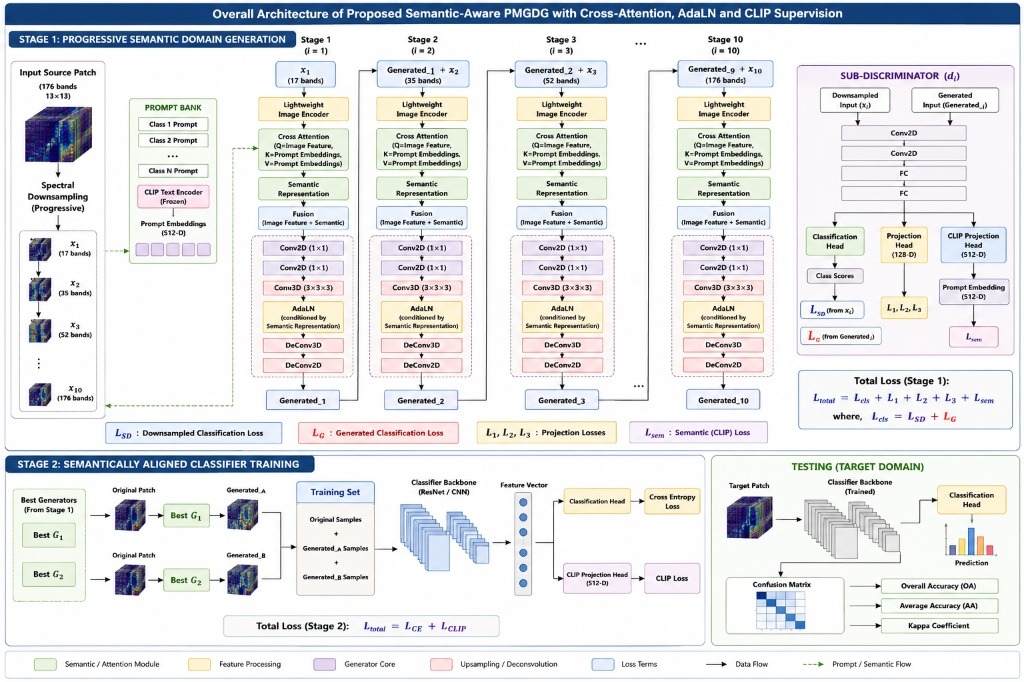
\includegraphics[width=0.95\textwidth]{architecture.jpg}
\caption{Detailed schematic flow of the proposed Semantic-Guided Progressive Domain Generalization framework. Stage 1 pre-trains progressive semantic-aware generators and discriminators on downsampled spectral steps. Stage 2 trains the final classifier on a joint set of original and generated patches using Sharpness-Aware Minimization (SAM) and cross-modal contrastive alignment.}
\label{fig:architecture}
\end{figure*}

\subsection{Problem Formulation}
To define the domain generalization task, we represent the spatial-spectral remote sensing datasets mathematically. Let the labeled source domain be denoted by $\mathcal{D}_S = \{(\mathbf{x}_i^s, y_i^s)\}_{i=1}^{N_S}$, where $N_S$ is the number of training samples, $\mathbf{x}_i^s \in \mathbb{R}^{H \times W \times C_s}$ represents the spatial-spectral HSI patch with spatial dimension $H \times W$ and spectral bands $C_s$, and $y_i^s \in \{1, 2, \dots, N_c\}$ is the class label among $N_c$ categories. Let the target domain be denoted by $\mathcal{D}_T = \{\mathbf{x}_j^t\}_{j=1}^{N_T}$. In our generalization setup, only source-domain data are used during training, and no target-domain information is accessed during optimization. The objective is to learn a mapping function $f: \mathbf{x} \to y$ that generalises to unseen target domain variations under domain shift:
\begin{equation}
\min_{f} \mathbb{E}_{\mathbf{x}^t, y^t \sim \mathcal{D}_T} \left[ \mathbb{I}(f(\mathbf{x}^t) \neq y^t) \right]
\end{equation}
where $\mathbb{I}(\cdot)$ is the indicator function, and $\mathbf{x}^t, y^t$ are samples from the unseen target distribution.

\subsection{Progressive Spectral Downsampling}
Due to the high dimensionality and spectral redundancy of HSIs, generating target-domain styles directly in a single step can lead to unstable training. To address this, we decompose the patch spectral bands into $K$ progressive stages. At each stage $k \in \{1, \dots, K\}$, the downsampling function $\Phi_k: \mathbb{R}^{H \times W \times C_s} \to \mathbb{R}^{H \times W \times C_k}$ averages adjacent spectral slices into $C_k$ groups, mapping the input patch $\mathbf{x}$ to a downsampled step $\mathbf{x}_k \in \mathbb{R}^{H \times W \times C_k}$:
\begin{equation}
\mathbf{x}_k(h, w, j) = \frac{1}{|S_j|} \sum_{c \in S_j} \mathbf{x}(h, w, c)
\end{equation}
where $S_j$ is the index set of the $j$-th spectral channel group, $|S_j|$ is the group size, and $C_1 < C_2 < \dots < C_K = C_s$.

\subsection{Semantic Guidance}
To guide style translation without altering the underlying category layout, we construct a Vision-Language Prompt Bank. The class category description $t_c$ is embedded using a frozen pre-trained CLIP text encoder $\mathbf{\Psi}_{text}$ into prompt embeddings $\mathbf{e}_c \in \mathbb{R}^{512}$:
\begin{equation}
\mathbf{e}_c = \mathbf{\Psi}_{text}(t_c)
\end{equation}
where $t_c$ represents the textual template corresponding to class $c$. To avoid redundant computation, these static embeddings are computed once and stored in the prompt matrix $\mathbf{E}_{txt} \in \mathbb{R}^{N_c \times 512}$.

\subsection{Semantic-Aware Progressive Generator}
At each stage $k$, the generator uses a visual-semantic pipeline to reconstruct the target HSI patch from the downsampled input $\mathbf{x}_k$.

\subsubsection{Multi-Head Cross Attention}
To associate spatial features with textual descriptions, query, key, and value representations are computed. The visual feature map $\mathbf{F}_{img} \in \mathbb{R}^{H \times W \times C_k}$ extracted from the lightweight encoder is flattened to sequence $\mathbf{F}_{flat} \in \mathbb{R}^{HW \times C_k}$ and projected to Queries, while class prompt embeddings $\mathbf{E}_{txt}$ are projected to Keys and Values:
\begin{equation}
\mathbf{Q} = \mathbf{F}_{flat} \mathbf{W}_Q, \quad \mathbf{K} = \mathbf{E}_{txt} \mathbf{W}_K, \quad \mathbf{V} = \mathbf{E}_{txt} \mathbf{W}_V
\end{equation}
where $\mathbf{W}_Q \in \mathbb{R}^{C_k \times d_{model}}$, $\mathbf{W}_K \in \mathbb{R}^{512 \times d_{model}}$, and $\mathbf{W}_V \in \mathbb{R}^{512 \times d_{model}}$ project features to dimension $d_{model} = 512$. Cross attention is formulated as:
\begin{equation}
\mathbf{F}_{attn} = \text{softmax}\left(\frac{\mathbf{Q} \mathbf{K}^T}{\sqrt{d_{model}}}\right) \mathbf{V} \mathbf{W}_O
\end{equation}
where $\mathbf{W}_O \in \mathbb{R}^{d_{model} \times C_k}$ is the output projection weight, and $\mathbf{F}_{attn} \in \mathbb{R}^{HW \times C_k}$ is the cross-attention output. Injecting semantic representations step-by-step prevents style-induced semantic drift.

\subsubsection{Semantic Fusion}
To combine visual textures and linguistic concepts dynamically, we use a gated fusion layer:
\begin{equation}
\mathbf{G} = \sigma\left(\left[\mathbf{F}_{flat} \parallel \mathbf{F}_{attn}\right] \mathbf{W}_{gate} + \mathbf{b}_{gate}\right)
\end{equation}
\begin{equation}
\mathbf{F}_{fusion} = \mathbf{F}_{img} + \alpha \cdot \text{Reshape}\left(\mathbf{G} \odot \mathbf{F}_{flat} + (\mathbf{1} - \mathbf{G}) \odot \mathbf{F}_{attn}\right)
\end{equation}
where $\mathbf{W}_{gate} \in \mathbb{R}^{2C_k \times C_k}$ and $\mathbf{b}_{gate} \in \mathbb{R}^{C_k}$ represent the gate weights and biases, $\sigma$ is the sigmoid function, $\alpha = 0.1$ is a learnable scaling parameter, and $\parallel$ is feature concatenation.

\subsubsection{Adaptive AdaLN}
To modulate intermediate HSI representation based on class semantics, we pool $\mathbf{F}_{sem}$ (the reshaped fused features) to semantic condition vector $\mathbf{v}_{sem} \in \mathbb{R}^{C_k}$ and project it to scaling $\mathbf{\gamma}$ and shifting $\mathbf{\beta}$ parameters:
\begin{equation}
\mathbf{\gamma}, \mathbf{\beta} = \text{Split}\left(\text{Linear}(\mathbf{v}_{sem})\right)
\end{equation}
The Adaptive Layer Normalization (AdaLN3d) operation on 3D intermediate backbone tensor $\mathbf{V}_{3D}$ is defined as:
\begin{equation}
\text{AdaLN3d}(\mathbf{V}_{3D}, \mathbf{v}_{sem}) = (\mathbf{1} + \mathbf{\gamma}) \odot \left(\frac{\mathbf{V}_{3D} - \mu(\mathbf{V}_{3D})}{\sqrt{\sigma^2(\mathbf{V}_{3D}) + \epsilon}}\right) + \mathbf{\beta}
\end{equation}
where $\mu$ and $\sigma^2$ denote the mean and variance computed over the channel dimension, and scale and shift are clamped to prevent gradient instability: $\mathbf{\gamma} = \text{clamp}(\mathbf{\gamma}, -0.9, 2.0)$ and $\mathbf{\beta} = \text{clamp}(\mathbf{\beta}, -3.0, 3.0)$.

\subsubsection{Progressive Reconstruction}
The fused spatial-spectral feature map is projected to PCA space via a $1 \times 1$ Conv2D, reshaped to a 3D volume, processed by Conv3D, normalized using AdaLN3d, upsampled with DeConv3D, and reconstructed to target spectral dimensions via a $1 \times 1$ Conv2D (DeConv2D):
\begin{equation}
\mathbf{x}_{gen} = \text{DeConv2D}\left(\text{DeConv3D}\left(\mathbf{V}_{norm}\right)\right)
\end{equation}
where $\mathbf{V}_{norm}$ is the AdaLN3d modulated feature map, and $\mathbf{x}_{gen} \in \mathbb{R}^{H \times W \times C_k}$ represents the generated target-style patch.

\subsection{Sub-Discriminator}
To evaluate the progressive multi-stage outputs, each stage $k$ utilizes a sub-discriminator $\mathbf{d}_k$ equipped with three heads: classification score head predicting class scores $\mathbf{p}_{cls}$, projection head mapping features to $\mathbf{z}_{proj} \in \mathbb{R}^{128}$, and CLIP projection head mapping features to $\mathbf{z}_{clip} \in \mathbb{R}^{512}$.

\subsection{Semantic Alignment}
To align the visual representations with prompt embeddings, we minimize a cross-modal contrastive classification loss over HSI patch CLIP projections and text prompt embeddings:
\begin{equation}
\mathcal{L}_{sem} = -\frac{1}{B} \sum_{i=1}^B \log \frac{\exp\left(\tau \cdot \mathbf{z}_{clip, i} \mathbf{e}_{y_i}^T\right)}{\sum_{j=1}^{N_c} \exp\left(\tau \cdot \mathbf{z}_{clip, i} \mathbf{e}_j^T\right)}
\end{equation}
where $\mathbf{z}_{clip, i}$ is the CLIP projection of the $i$-th HSI patch in a batch of size $B$, $\mathbf{e}_{y_i}$ is the prompt embedding of the ground-truth class, and $\tau$ is a temperature scaling parameter.

\subsection{Two-Stage Training}
\subsubsection{Stage 1: Generator Pre-training}
During Stage 1, we optimize the progressive generators and sub-discriminators. We define the general contrastive loss $\mathcal{L}_{con}$ for a batch $I$ with views $A(i)$ and class mates $P(i)$ as:
\begin{equation}
\mathcal{L}_{con}(\mathbf{Z}, y, adv) = \sum_{i \in I} \frac{-1}{|P(i)|} \sum_{p \in P(i)} \log \Psi(i, p, adv)
\end{equation}
where $\Psi(i, p, adv)$ represents the alignment probability:
\begin{equation}
\Psi(i, p, adv) = \begin{cases}
    \frac{\exp(\mathbf{z}_i \cdot \mathbf{z}_p / \tau)}{\sum_{a \in A(i)} \exp(\mathbf{z}_i \cdot \mathbf{z}_a / \tau)} & adv=\text{False} \\
    1 - \frac{\exp(\mathbf{z}_i \cdot \mathbf{z}_p / \tau)}{\sum_{a \in A(i)} \exp(\mathbf{z}_i \cdot \mathbf{z}_a / \tau)} & adv=\text{True}
\end{cases}
\end{equation}
The downsampled consistency loss $\mathcal{L}_{wd}$ aligns original features $\mathbf{z}_{whole}$ and PCA-downsampled features $\mathbf{z}_{down}$:
\begin{equation}
\mathcal{L}_{wd} = \mathcal{L}_{con}([\mathbf{z}_{whole} \parallel \mathbf{z}_{down}], y, \text{False})
\end{equation}
The total discriminator loss at stage $k$ is:
\begin{equation}
\mathcal{L}_{total}^D = \mathcal{L}_{SD} + \lambda_1 \mathcal{L}_{1} + \lambda_{sem} \mathcal{L}_{sem}^D
\end{equation}
where $\mathcal{L}_{SD} = \mathcal{L}_{CE}(\mathbf{p}_{down}, y) + \mathcal{L}_{CE}(\mathbf{p}_{gen}, y)$ evaluates class correctness, and $\mathcal{L}_1$ is the interclass projection contrastive loss computed using $\mathcal{L}_{con}$. The generator is trained using:
\begin{equation}
\mathcal{L}_{total}^G = \mathcal{L}_{G} + \lambda_2 \mathcal{L}_{2} + \lambda_{sem} \mathcal{L}_{sem}^G
\end{equation}
where $\mathcal{L}_2$ is the intraclass adversarial contrastive loss, and $\mathcal{L}_G = \mathcal{L}_{CE}(\mathbf{p}_{gen}, y)$.

\subsubsection{Stage 2: Classifier Training}
The pre-trained generators $G_1, G_2$ are frozen to construct a joint training set of original source patches and synthesized target variations:
\begin{equation}
\mathbf{X}_{train} = \left[\mathbf{x} \parallel G_1(\mathbf{x}) \parallel G_2(\mathbf{x})\right]
\end{equation}
The final classifier parameters $\theta$ are trained using SAM. SAM searches for parameters in flat loss regions:
\begin{equation}
\theta \leftarrow \theta - \eta \nabla_{\theta} \mathcal{L}_{Stage2}(\theta + \epsilon(\theta))
\end{equation}
where $\epsilon(\theta) = \arg\max_{\|\epsilon\| \le \rho} \mathcal{L}_{Stage2}(\theta + \epsilon)$, and $\rho$ is the perturbation radius. The Stage 2 joint loss is formulated as:
\begin{equation}
\mathcal{L}_{Stage2} = \mathcal{L}_{CE}(\mathbf{p}_{cls}, y_{total}) + \lambda_{clip} \mathcal{L}_{clip}
\end{equation}
where $\mathcal{L}_{clip}$ is the contrastive CLIP loss computed over the expanded batch of size $3B$:
\begin{equation}
\mathcal{L}_{clip} = -\frac{1}{3B} \sum_{i=1}^{3B} \log \frac{\exp\left(\tau \cdot \mathbf{z}_{clip, i} \mathbf{e}_{y_{total, i}}^T\right)}{\sum_{j=1}^{N_c} \exp\left(\tau \cdot \mathbf{z}_{clip, i} \mathbf{e}_j^T\right)}
\end{equation}

\subsection{Testing / Inference}
During testing, generators are discarded. Inference is performed directly on unseen target HSI patches $\mathbf{x}^t \in \mathcal{D}_T$ using the classifier backbone to calculate classification accuracy. No target-domain images are accessed during training. Evaluation is performed using Overall Accuracy (OA), Average Accuracy (AA), and the Kappa coefficient.

\subsection{Training Algorithm}
\label{sec:algorithm}

Algorithm~\ref{alg:training} summarizes the complete two-stage training procedure of the proposed SG-PMG framework.

\begin{algorithm}[H]
\caption{Two-Stage Training Procedure of SG-PMG}
\label{alg:training}
\begin{algorithmic}[1]
\REQUIRE Source dataset $\mathcal{D}_s = \{(\mathbf{x}_i, y_i)\}$, Target dataset $\mathcal{D}_t = \{\mathbf{x}_j^t\}$, target class prompt bank $\mathbf{E}_{txt}$, batch size $B$, stage epochs $E_1, E_2$, progressive steps $K$, scaling weights $\lambda_1, \lambda_2, \lambda_{sem}, \lambda_{clip}$.
\ENSURE Optimized classifier $D_{net}$.

\STATE Load CLIP model on device; compute cached text features $\mathbf{E}_{txt}$.
\STATE Initialize progressive networks $g_1, g_2, d_1, d_2$.

\STATE \COMMENT{\textbf{STAGE 1: Progressive Generator Pre-training}}
\FOR{epoch = 1 \TO $E_1 \cdot K$}
    \STATE Calculate current progressive step: $k = \lfloor \text{epoch}/E_1 \rfloor + 1$.
    \FOR{each mini-batch $(\mathbf{X}, \mathbf{y}) \in \mathcal{D}_s$}
        \STATE Extract class prompts: $\mathbf{e}_y = \text{Index}(\mathbf{E}_{txt}, \mathbf{y})$.
        \STATE $\mathbf{X}_g, \mathbf{X}_{down} \leftarrow \text{Forward}(g_1, \mathbf{X}, k, \mathbf{e}_y, \mathbf{E}_{txt})$.
        \STATE Compute downsampled consistency loss: $\mathcal{L}_{wd} \leftarrow \mathcal{L}_{con}([\mathbf{z}_{whole} \parallel \mathbf{z}_{down}], \mathbf{y})$.
        \STATE Compute discriminator loss $\mathcal{L}_{1\_1}$ using class and semantic losses.
        \STATE Compute generator style adversarial loss: $\mathcal{L}_{2\_1} \leftarrow \text{CE}(\mathbf{p}_{tgt}, \mathbf{y}) + \lambda_2 \mathcal{L}_{adv} + \lambda_{sem} \mathcal{L}_{sem}$.
        \STATE Update $d_1$ and $g_1$ parameters using Adam optimizers.
        \STATE Repeat updates for $d_2$ and $g_2$.
    \ENDFOR
\ENDFOR

\STATE \COMMENT{\textbf{STAGE 2: SAM-Guided Classifier Tuning}}
\STATE Initialize standalone classifier $D_{net}$; load weights from the final pre-trained sub-discriminator $d_1[-1]$.
\FOR{epoch = 1 \TO $E_2$}
    \FOR{each mini-batch $(\mathbf{X}, \mathbf{y}) \in \mathcal{D}_s$}
        \STATE $\mathbf{X}_1 \leftarrow g_1(\mathbf{X}, K, \mathbf{e}_y)$, $\mathbf{X}_2 \leftarrow g_2(\mathbf{X}, K, \mathbf{e}_y)$ (in evaluation mode).
        \STATE Concatenate tensors: $\mathbf{X}_{total} \leftarrow [\mathbf{X} \parallel \mathbf{X}_1 \parallel \mathbf{X}_2]^T$, $\mathbf{y}_{total} \leftarrow [\mathbf{y} \parallel \mathbf{y} \parallel \mathbf{y}]^T$.
        \STATE $\mathbf{p}, \mathbf{z}_{clip} \leftarrow D_{net}(\mathbf{X}_{total})$.
        \STATE Compute classification and CLIP semantic losses: $\mathcal{L} \leftarrow \text{CE}(\mathbf{p}, \mathbf{y}_{total}) + \lambda_{clip} \mathcal{L}_{clip}(\mathbf{z}_{clip}, \mathbf{y}_{total})$.
        \STATE Backward pass: Compute gradients $\mathbf{g} = \nabla_{\mathbf{w}} \mathcal{L}$.
        \STATE Compute SAM parameter perturbation: $\mathbf{\epsilon} = \rho \frac{\mathbf{g}}{\|\mathbf{g}\|_2}$.
        \STATE Shift parameters: $\mathbf{w} \leftarrow \mathbf{w} + \mathbf{\epsilon}$.
        \STATE Re-evaluate loss on shifted parameters: $\mathcal{L}_{sharp} \leftarrow D_{net}(\mathbf{X}_{total})$.
        \STATE Backward pass: Compute gradients $\mathbf{g}_{sharp} = \nabla_{\mathbf{w}} \mathcal{L}_{sharp}$.
        \STATE Update parameters: $\mathbf{w} \leftarrow \mathbf{w} - \eta \cdot \mathbf{g}_{sharp}$.
    \ENDFOR
\ENDFOR
\RETURN $D_{net}$.
\end{algorithmic}
\end{algorithm}

